\newpage
\hypertarget{conBran tex}{}
\subsection{Branching with statement nodes}
\texHeader

\begin{itemize}

\item[$\blacktriangleright$] Before doing anything else, let's declare the method that will insert two new partitions into \texttt{box} when the original
pattern match fails. Open \texttt{Box.eclass} and add the following signature: 
\syntax{initializeBox () : EBoolean}

\vspace{0.5cm}

\item[$\blacktriangleright$] Now we modify \texttt{Box.grow()} by adding a nested \emph{if/else} construct, with \texttt{[addNewPartitionBox]} as the
first conditional, and a statement node as the second. \texttt{grow} should now resemble Fig.~\ref{fig:updateGrow}

\vspace{0.5cm}

\begin{figure}[htp]
\begin{center}
  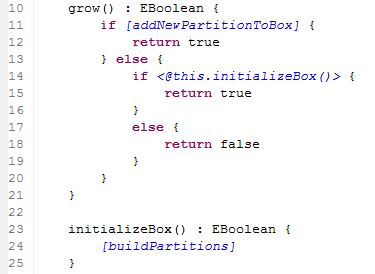
\includegraphics[width=0.5\textwidth]{eclipse_updateGrow}
  \caption{Our first \emph{statement node}}
  \label{fig:updateGrow}
\end{center}
\end{figure}

\vspace{0.5cm}

\item[$\blacktriangleright$] Easy! Now, we want to specify our newest method. As we mentioned before, you now have a choice -- you can either write the Java
implementation yourself in \texttt{Box.impl}, or continue with a pattern. Given that this method is pretty structural, it should work beautifully as a pattern.
Let's call the new pattern \texttt{buildPartitions}

\vspace{0.5cm}

\item[$\blacktriangleright$] Open and complete \texttt{[buildPartitions]} as illustrated in Fig.~\ref{fig:pattBuildParts}. As you can see, we have a bound
box to check and see if a connection to \texttt{onePartition} exists. If none exists, the pattern will proceed to create a \texttt{firstPartition} and
\texttt{lastPartition}, and connect them accordingly.

\clearpage

\vspace*{2cm}

\begin{figure}[htp]
\begin{center}
  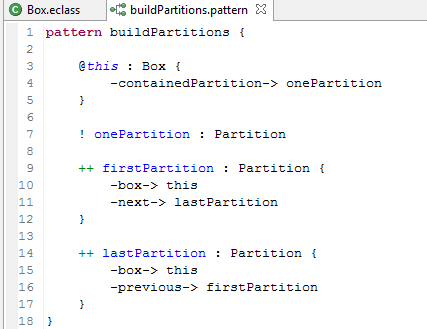
\includegraphics[width=0.7\textwidth]{eclipse_buildPartitionsPattern}
  \caption{Pattern to initalize the box, but only if it's empty \update}
  \label{fig:pattBuildParts}
\end{center}
\end{figure}

\item[$\blacktriangleright$] That's it! Save and build your metamodel to make sure no errors exist.

\end{itemize}
